\chapter*{Lab 2 - Modelli Geometrici 3D}

\section{Caricamento e visualizzazione modelli geometrici}
Il primo punto dell'esercitazione richiedeva di implementare le seguenti funzioni:
\begin{enumerate}
  \item Caricamento e visualizzazione modelli geometrici di tipo mesh in formato .m
  \item Visualizzazione superfici quadriche dalla libreria GLU (es. Sfere, cilindri, tori)
  \item Verifica della gestione della visualizzazione dei modelli poligonali a mesh tramite display list.
  \item Calcolo e memorizzazione delle normali ai vertici per i modelli mesh poligonali. Visualizzazione con normali ai vertici in modalità smooth.
\end{enumerate}

I punti 1 3 e 4 sono stati applicati nella funzione \texttt{loadMesh()} che viene richiamata nel main un numero di volte pari a MESH, una costante dell'applicativo fissata a 4 che rappresenta il numero di oggetti da disegnare. Nel main viene quindi generata una display list per ogni oggetto, riempita opportunamente nella funzione \texttt{loadMesh()} con le informazioni necessarie per disegnarlo. Gli oggetti sono stati scelti dalla cartella \texttt{../data} presente nel template dell'esercitazione e sono \textit{pig.m}, \textit{cactus.m}, \textit{teapot.m}.

La funzione \texttt{loadMesh()} è stata creata sulla base della funzione \texttt{init()} già presente nel template ed esegue nell'ordine:
\begin{itemize}
  \item apertura del file *.m
  \item lettura di tutte le linee e quindi vertici e facce dell'oggetto
  \item per ogni faccia viene eseguito il calcolo della normale alla faccia
  \item per ogni vertice eseguito il calcolo della normale al vertice
  \item chiusura del file
  \item inizializzazione della display list relativa all'oggetto e riempimento di essa con il disegno di ogni triangolo della mesh.
\end{itemize}
\newpage
\subsection{Normale alla faccia}

\begin{wrapfigure}{l}{0.4\textwidth}
    \centering
    \vspace{-0.5cm}
    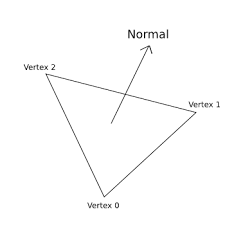
\includegraphics[height=5.5cm]{face}
    \caption{\label{fig:face}}
    \vspace{-0.5cm}
\end{wrapfigure}
Ogni faccia è costituita da 3 vertici poiché ogni faccia è un triangolo. La normale alla faccia è ottenuta attraverso la cross-correlazione di due vettori ottenuti dalle sottrazioni $v_2 - v_0$ e $v_1 - v_0$. Il risultato della cross-correlazione viene poi normalizzato ottenendo la normale alla faccia: 
\begin{itemize}
  \item $v_a = v_2 - v_0$
  \item $v_b = v_1 - v_0$
  \item $norm = cross\_product(v_a, v_b)$
  \item $normalize(norm)$
\end{itemize}

Questi passaggi sono stati applicati nel codice attraverso le funzioni già presenti nella libreria \texttt{v3d.h}

\subsection{Normale al vertice}

\begin{wrapfigure}{l}{0.4\textwidth}
    \centering
    \vspace{-0.5cm}
    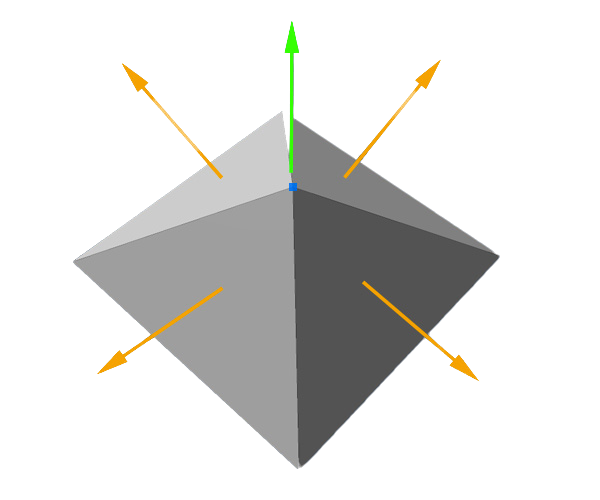
\includegraphics[height=5.5cm]{vertex}
    \caption{\label{fig:vertex}}
    \vspace{-0.5cm}
\end{wrapfigure}

La normale al vertice è ottenuta calcolando la media di tutte le normali. I passi implementati nel codice sono i seguenti:\\

\noindent Per ogni vertice $i$: 
  	 \begin{itemize}
  			  \item Crea vettore somma $S$
  			\item Crea contatore $k$
  			\item Per ogni faccia $j$:
  				\begin{itemize}
  					\item Se la faccia $j$ contiene il vertice $i$ allora somma ad $S$ la normale alla faccia e incrementa il contatore $k$
  				\end{itemize}
  			\item dividi $S$ per $k$
  			\item normalizza $S$
		\end{itemize}

\newpage
\section{Controllo interattivo della scena}
Le funzioni da implementare erano le seguenti:
\textbf{
\begin{itemize}
  \item Zoom
  \item Proiezione
  \item Culling
  \item Wireframe
  \item Shading
  \item Sistemare movimento della TrackBall
  \item Esplorazione della scena tramite un'animazione.
\end{itemize}}

\subsection{Zoom}
Lo zoom è stato implementato in due modi:
\begin{itemize}
  \item \textbf{tramite l'utilizzo della funzione richiamabile dal menu a tendina (con f,F)}: nella funzione \texttt{keyboard()} sono stati aggiunti due \textit{case} per la pressione dei tasti 'f' e 'F'. Il risultato è la variazione del parametro \textit{fovy} ovvero il \textit{field of view} della camera.
  \item \textbf{tramite lo scorrimento della rotellina del mouse (o del trackpad)}: il principio è lo stesso di quello sopra, ma occorre aggiungere al main la primitiva \texttt{glutMouse\-Wheel\-Func\-(mouseWheel);} che richiama appunto la \textit{mouseWheel()} ad ogni scorrimento della rotellina del mouse.
\end{itemize}

\subsection{Proiezione}
Attraverso la variabile globale \textit{orpro} si tiene conto di quale sia la proiezione corrente. Nella \texttt{display()} sotto alla \texttt{glMatrixMode(GL\_PROJECTION)}, si applica la ortografica o la prospettiva a seconda di \textit{orpro}:

\begin{itemize}
  \item se \textit{vera}: si usa la funzione \texttt{
		glOrtho(-fovr, fovr, -fovr, fovr, -fovr, fovy)} inserendo i valori dei piani di clipping relativi al \textit{field of view} della camera. In questo modo è possibile usare lo zoom anche in ortografica poiché i piani di clipping variano in base al parametro \textit{fovr} che si basa sul valore di \textit{fovy}
  \item se \textit{falsa}: si usa la funzione \texttt{
		gluPerspective(fovy, aspect, 1, 100);}
\end{itemize}
\begin{figure}[hbt]%
	\vspace{-1cm}
    \centering
    \subfloat[Ortografica]{{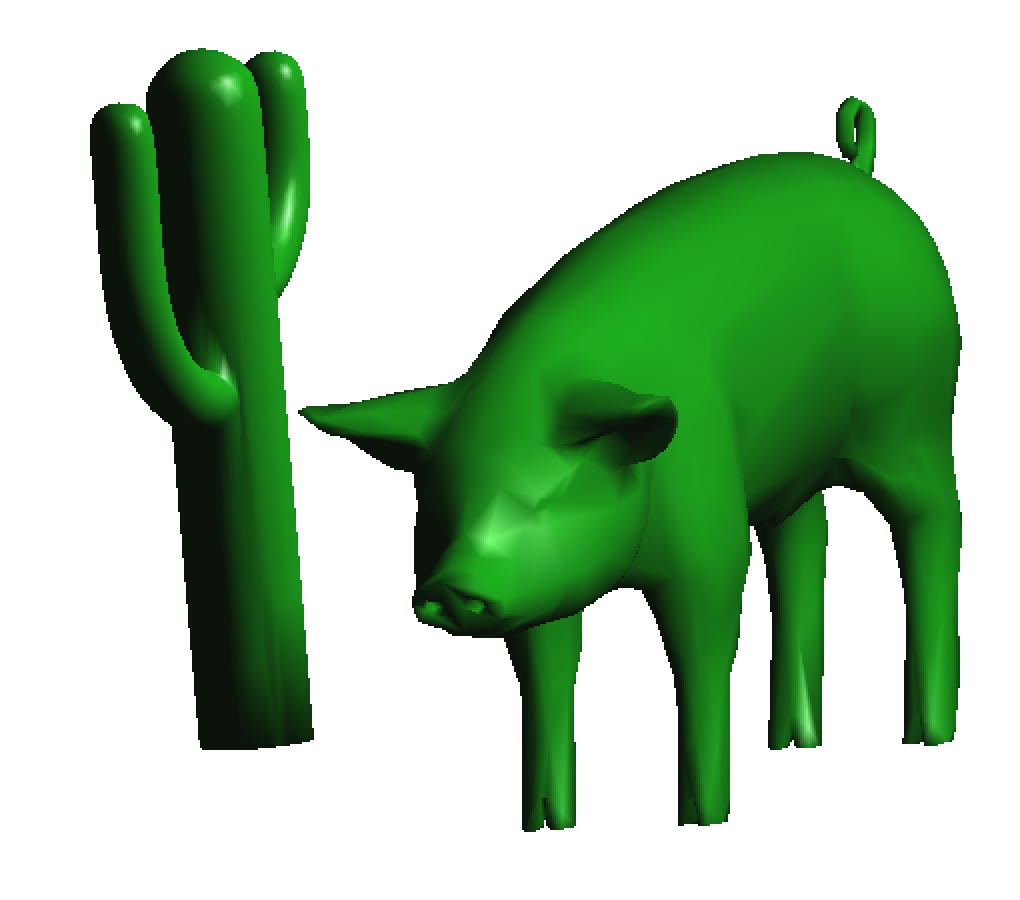
\includegraphics[height=4cm]{ortho} }}%
    \subfloat[Prospettiva]{{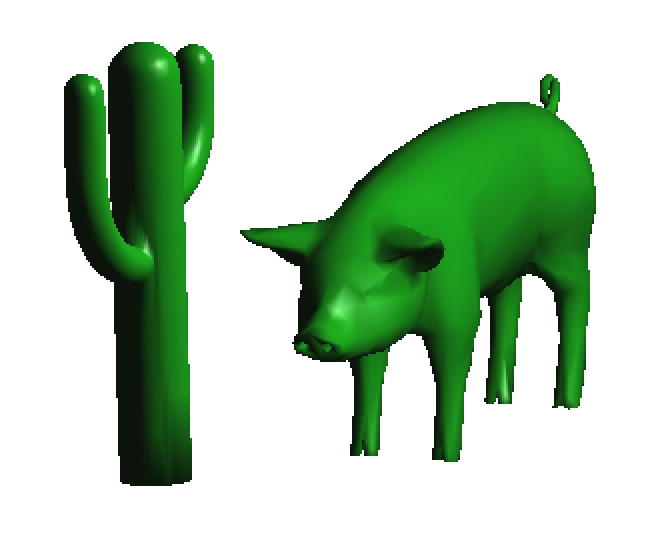
\includegraphics[height=4cm]{prosp} }}%
	\vspace{-0.2cm}
\end{figure}

Come si può notare, nella prospettiva il maialino ha una dimensione minore, mentre nell'ortografica si ha una proiezione parallela e quindi le dimensioni rimangono le stesse.

\subsection{Culling, Wireframe, Shading}
Queste tre funzioni sono state abilitate nella funzione \texttt{display} a seconda del corrispettivo parametro intero che ne determina l'abilitazione. Le tre sono state abilitate grazie alle primitive: 
\begin{itemize}
  \item \textbf{Culling}: abilitata con \texttt{glEnable\-(GL\_CULL\_FACE)} e disabilitata con \texttt{glDisable\-(GL\_CULL\_FACE)}
  \item \textbf{Wireframe}: abilitata con \texttt{glPolygon\-Mode\-(GL\_FRONT\_AND\_BACK, GL\_LINE)} e disabilitata con \texttt{glPolygon\-Mode\-(GL\_FRONT\_AND\_BACK, GL\_FILL)}
  \item \textbf{Shading}: abilitato con \texttt{glShadeModel\-(GL\_SMOOTH)} e disabilitato con \texttt{glShadeModel\-(GL\_FLAT)}
\end{itemize}

\begin{figure}[hbt]%
	\vspace{-1cm}
    \centering
    \subfloat[Wireframe ON]{{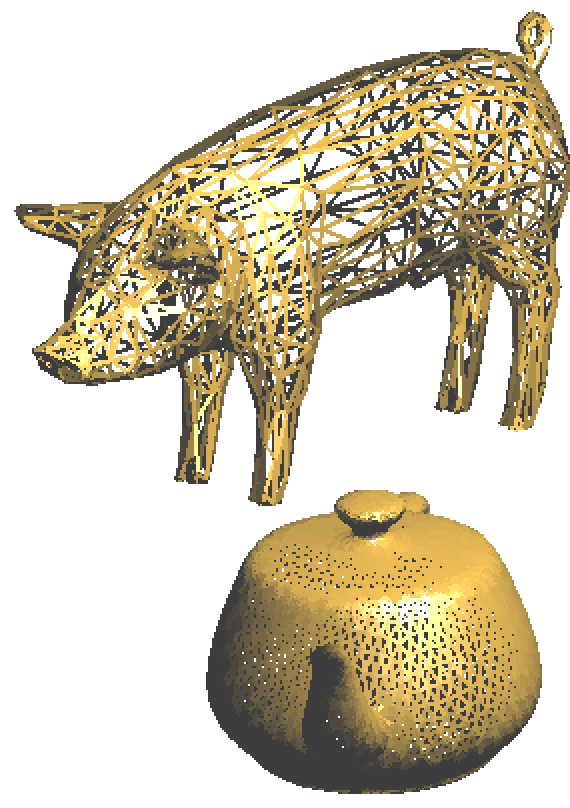
\includegraphics[height=4cm]{wireframe} }}%
    \subfloat[Culling ON]{{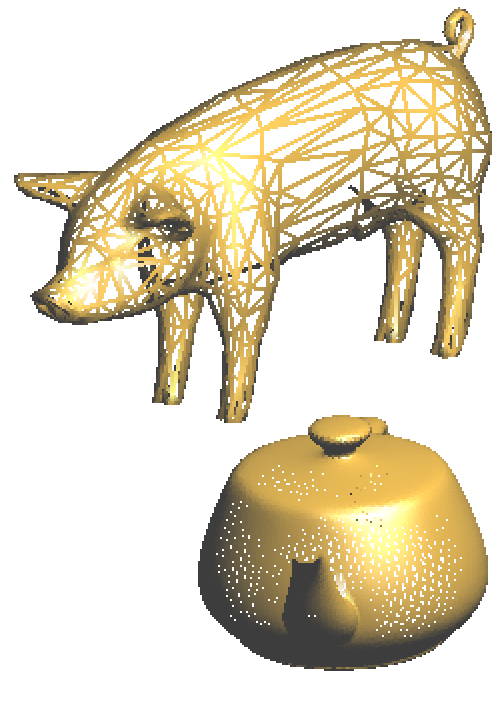
\includegraphics[height=4cm]{culling} }}%
 	\subfloat[Shading Flat]{{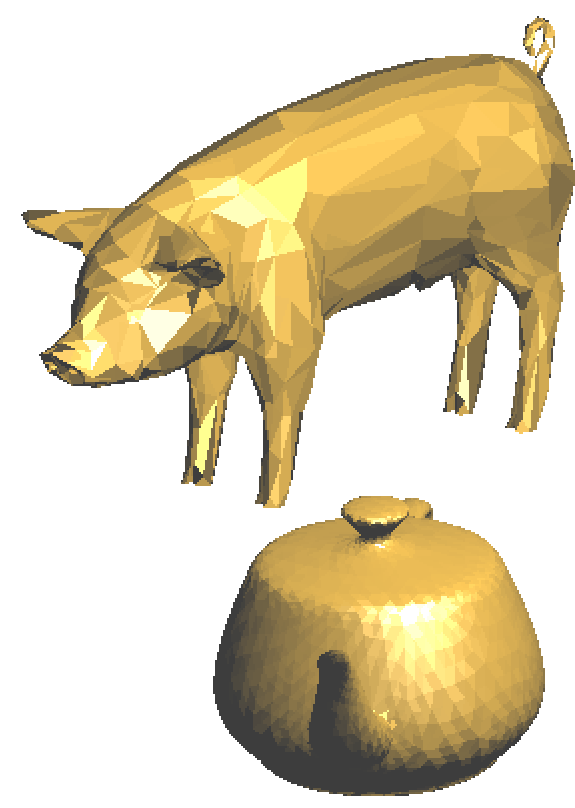
\includegraphics[height=4cm]{shadingoff} }}
    \subfloat[Shading Smooth]{{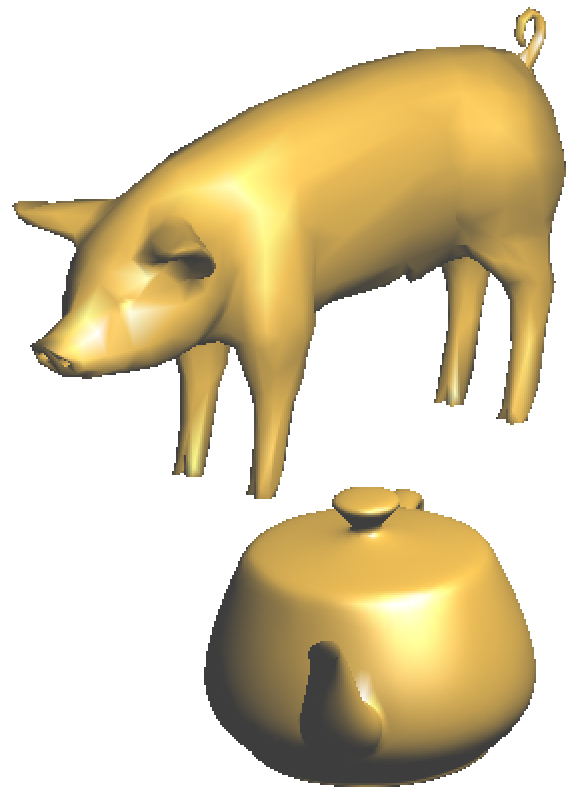
\includegraphics[height=4cm]{shadingon} }}
	\vspace{-0.2cm}
\end{figure}

Nell'immagine Culling ON si può notare che le facce interne non vengono visualizzate, in quanto il culling viene abilitato a default per GL\_BACK, ovvero il retro delle facce.

\subsection{Camera Motion}

Per fare in modo che la telecamera seguisse una traiettoria attorno alla scena è  necessario creare una curva di Bézier chiusa a coordinata Y costante. Dati alcuni punti di controllo che creano la curva e applicando l'algoritmo di De Casteljau usato nella prima esercitazione, è bastato abilitare la funzione \texttt{idle()} con un incremento del parametro t ogni 50 millisecondi e una chiamata alla routine \texttt{moveCamera()} che applica l'algoritmo di De Casteljau. Ogni punto trovato con l'algoritmo sarà assegnato al punto C della camera, ovvero l'occhio della camera (eye). La funzione è selezionabile dal menù a tendina e l'effetto finale è un'animazione che sorvola la scena. 

\subsection{Trackball}
La trackball è stata implementata in due modi diversi, ma solo il secondo modo ha portato ad una rotazione corretta. Per completezza riporto entrambi i metodi.
\begin{itemize}
  \item \textbf{Primo metodo}: nella funzione \texttt{motion()} si mantiene in memoria l'ultima rotazione e l'ultima posizione relativa degli assi. Basta applicare l'operatore $+=$ ad \textit{tbAngle} e \textit{tbAxis} e ad ogni movimento aggiornare l'ultima posizione con \texttt{v3dSet(lastPosition,\- currentPosition);} dove \textit{lastPosition} e \textit{currentPosition} sono rispettivamente \textit{tbW} e \textit{tbV}. Questo metodo permette di salvare l'ultima posizione della trackball e continuare la rotazione, ma questa avviene sempre ad un angolo positivo e non permette mai di cambiare direzione di rotazione. Questo metodo è stato mantenuto fino al completamento del terzo punto, il quale ha permesso di comprendere meglio il funzionamento dello stack delle matrici e di applicare quando imparato anche alla rotazione della trackball.
  \item \textbf{Secondo metodo}: si basa sul concetto che ad ogni trascinamento, prima viene calcolato ciò che riguarda la rotazione e poi viene disegnato il risultato. Si sfrutta questo concetto nella \texttt{motion()} creando la matrice di rotazione della trackball che verrà poi applicata nella \texttt{display()} moltiplicandola alla fine di tutto (quindi in cima ad ogni altra operazione sullo stack delle matrici di trasformazione) con la \texttt{glMultMatrixf\-(WCS[TRACKBALL])}. Il codice è il seguente:
  \begin{lstlisting}
  	glLoadIdentity();
	glRotatef(tbAngle, tbAxis[0], tbAxis[1], tbAxis[2]);
	glMultMatrixf(WCS[TRACKBALL]);
	glGetFloatv(GL_MODELVIEW_MATRIX, WCS[TRACKBALL]);
  \end{lstlisting}
\end{itemize}
Ulteriori dettagli sulla sequenza di queste operazioni saranno dati nella sezione che segue.

\section{Manipolazione dello stack delle matrici di trasformazione}
Le funzioni richieste sono state aggiunte al menù e alla funzione \texttt{keyboard()}. Ciò che verrà trattato in dettaglio riguarda la serie di operazioni eseguite sulle matrici di trasformazione per ottenere traslazioni e rotazioni attorno a OCS e WCS. È necessario distinguere i due casi in cui applicando una trasformazione, questa venga applicata in OCS o in WCS.

Per questo punto si è fatto uso di 3 matrici per mantenere lo stato di ogni oggetto (compresa la trackball):
\begin{itemize}
  \item \texttt{WCS[MESH][16]}: matrice che contiene lo stato delle trasformazioni di ogni oggetto rispetto al sistema di riferimento della scena
  \item  \texttt{OCS[MESH][16]}: matrice che contiene lo stato delle trasformazioni di ogni oggetto rispetto al proprio sistema di riferimento
  \item  \texttt{initialPosition[MESH][16]}: matrice che contiene la posizione iniziale di ogni oggetto.
\end{itemize}

Le prime due matrici vengono aggiornate ogni volta che l'utente seleziona traslazione o rotazione rispetto a WCS o OCS. Questa modifica viene effettuata nella funzione \texttt{keyboard()} ogni volta che l'utente preme $x$,$y$,$z$ richiamando la funzione \texttt{applyTransform()}. Questa funzione, analogamente a ciò che avviene per la trackball, carica una matrice identità, moltiplica per la matrice precedente (che rappresenta la posizione precedente dell'oggetto) e applica la nuova traslazione o rotazione. Ovviamente la funzione distingue i casi in cui l'utente abbia selezionato OCS o WCS e traslazione e rotazione.

Questa applicazione permette di non \textit{sporcare} la \texttt{display()} con rotazioni e traslazioni e permette di applicare sempre la stessa sequenza di operazioni. Per ogni mesh della scena si applicano le seguenti operazioni:
\begin{itemize}
  \item \texttt{glPushMatrix()} : rilevo dallo stack una copia della matrice attuale applicando le seguenti operazioni solo a ciò che viene disegnato all'interno della push e della pop.
  \item \texttt{glMultMatrixf(WCS[mesh])} : applico le trasformazioni rispetto al WCS
  \item \texttt{glMultMatrixf(initialPosition[mesh])} : applico la posizione iniziale rispetto al WCS
  \item \texttt{drawAxis(1, 0)} : disegno gli assi nella posizione iniziale dell'oggetto
  \item \texttt{glMultMatrixf(OCS[mesh])} : applico le trasformazioni rispetto all'OCS
  \item \texttt{glCallList(mesh)} : disegno l'oggetto nella posizione derivante da WCS, posizione iniziale, OCS

  \item \texttt{glPopMatrix()} applico le modifiche allo stack
\end{itemize}
 \begin{figure}[htb]
    \centering
    \vspace{-0.7cm}
    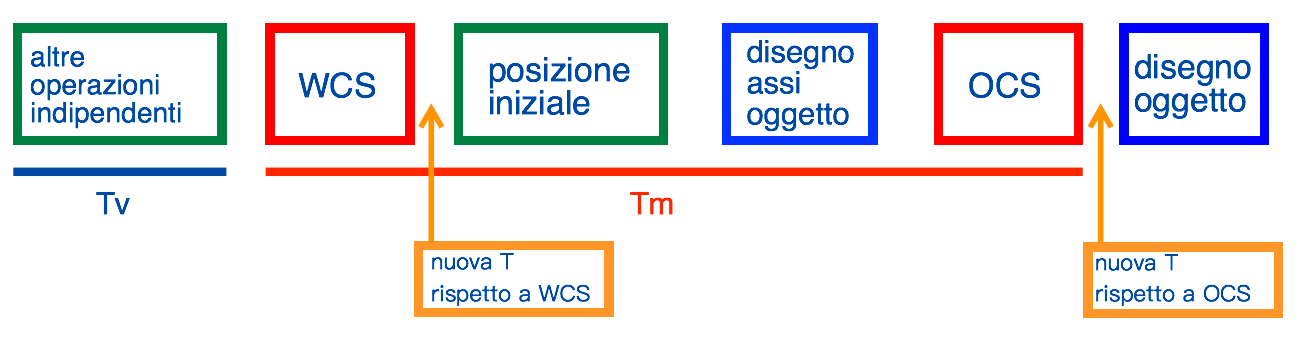
\includegraphics[width=\textwidth]{diagramma}
    \caption*{\label{fig:diagramma}}
    \vspace{-0.3cm}
\end{figure}

Un esempio del risultato finale, con gli oggetti nella posizione iniziale. Per visualizzare gli assi, è necessario utilizzare la funzione DEBUG del menù a tendina.
 \begin{figure}[htb]
    \centering
    %\vspace{-0.7cm}
    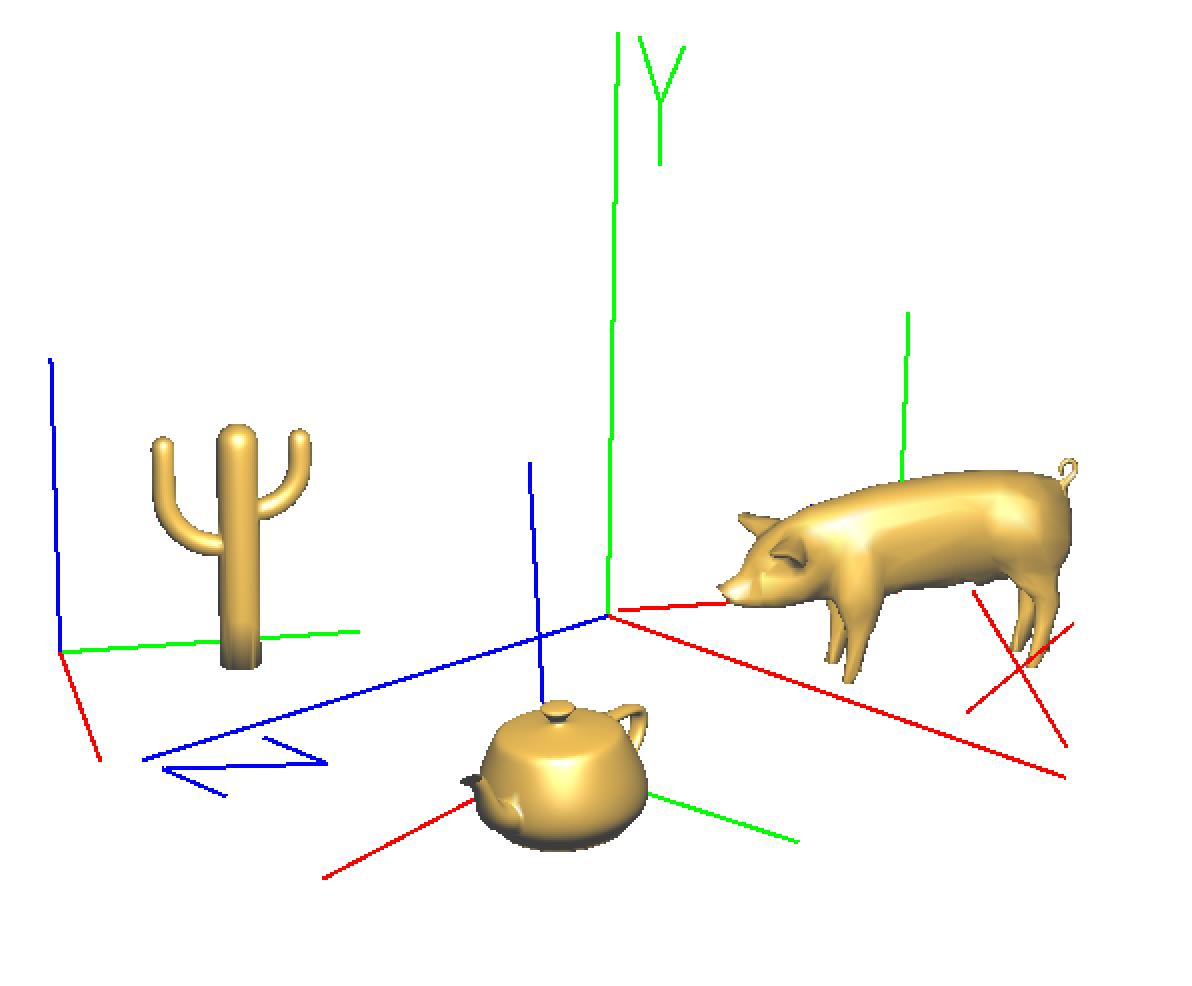
\includegraphics[width=0.8\textwidth]{result}
    \caption*{\label{fig:result}}
    %\vspace{-0.3cm}
\end{figure}


Note: 
\begin{itemize}
  \item è stata creata una funzione che inizializza i colori \texttt{initColors()}, in modo da rendere più leggibile il codice nella \texttt{display()}
  \item si è scelto di fissare la luce in modo tale che fosse solidale alla trackball.
\end{itemize}









%